\chapter{Defect chemistry and \ce{Li} ion diffusion in \ce{Li4Mn2O5}}
\section{Background}
As discussed in Chapter 1, there has been recent interest in disordered rock-salts as next generation cathode materials.
\ce{Li4Mn2O5}, one such material, offers capacities (\SI{355}{\milli\ampere\hour\per\gram}) which far exceed those seen in conventional cathodes, and uses non-toxic and earth-abundant manganese in place of cobalt.

This section consists of the first atomistic and defect and dynamics studies of \ce{Li4Mn2O5}, addressing issues arising due to the highly disordered nature of the material.
\newpage
\begin{figure}
\centering
\includegraphics[width=0.7\linewidth]{figures/structures/Li4Mn2O5}
\caption[Crystal structure of \ce{Li4Mn2O5}]{Crystal structure of \ce{Li4Mn2O5}. Li ions: green; Mn ions: purple; \ce{O} ions: red.}
\label{fig:Li4Mn2O5-average}
\end{figure}
\section{Structure generation and modelling}
\ce{Li4Mn2O5}, shown in Figure \ref{fig:Li4Mn2O5-average}, has an average \ce{MnO} rock-salt structure with the random substitution of 2/\nth{3}\textsuperscript{s} of \ce{Mn} sites with Li, charge compensated by 1/\nth{6} of oxygen sites being vacant.
While no ordering is noted in experimental work,\cite{Freire2016,Diaz-Lopez2018a} computational studies have identified a number of ordered structures which lower energies than pseudo-random structures generated for comparison.\cite{Diaz-Lopez2017,Bhandari2019}

\newpage
\subsection{Mean-field approximation}
The mean-field approximation can be used to study systems with partially occupied sites without the need to assign either a vacancy or given species to each site.
This is a useful exercise for the purposes of validating potential parameters against experimental lattice parameters.
The potential parameters used to study this system were taken from past work in literature on lithium manganese oxides by \citet{Ammundsen1999}, and are listed in Table \ref{tab:potentials}.
As GULP cannot implement the core-shell model for systems with multiple species occupying a given site, a rigid-ion model is used here.

The lattice parameters calculated give good agreement with experimental work, within $2.5\%$ of experimental work, although it is noted in literature that local deviations from the rock-salt structure arising from structural disorder give rise to a broad range of interatomic spacings, which this model cannot replicate.\cite{Yahia2019}

\begin{table}[h]
\centering
\caption[Two-body short-range potential parameters for \ce{Li4Mn2O5}]{Two-body short-range potential parameters for \ce{Li4Mn2O5}.\cite{Ammundsen1999}}
\begin{tabular}{@{}lS[table-format=5.2]S[table-format=1.4]S[table-format=2.1]S[table-format=1.2]S[table-format=5.1]@{}}
\toprule
\textbf{Interaction} &\multicolumn{1}{c}{\textbf{A} (\si{\electronvolt})}   & \multicolumn{1}{c}{$\boldsymbol{\rho}$ (\AA)} & \multicolumn{1}{c}{\textbf{C} (\si{\electronvolt \angstrom \tothe{6}})} & \multicolumn{1}{c}{\textbf{Y} (e)}& \multicolumn{1}{c}{\textbf{K} (\si{\electronvolt \angstrom \tothe{-2}})}\\
\midrule
\ce{Li+ -\;O^2-}   & 426.48  & 0.300                          & 0.0  & 1.0        & 99999.0 \\
\ce{Mn^3+ -\;O^2-}       & 1267.5  & 0.3240                         & 0.0  & 3.00       & 850.0   \\
\ce{O^2- -\;O^2-}        & 22764.3 & 0.1490                         & 43.0 & -2.96      & 57.0\\
\bottomrule
\end{tabular}
\label{tab:potentials}
\end{table}


\newcommand{\tableline}{\multicolumn{1}{c}{--}}
\newcommand{\tableliner}{\multicolumn{1}{c}{{\color{red}--}}}
\newcommand{\mc}[1]{\multicolumn{1}{c}{#1}}

\begin{table}[h]
\centering
\caption{Calculated lattice parameters of \ce{Li4Mn2O5} using mean-field approximation compared to experimental data.}
\begin{tabular}{lS[table-format=1.4]S[table-format=1.4]S[table-format=1.4]S[table-format=2.1]S[table-format=2.1]S[table-format=2.1]}
\toprule
\textbf{Lattice parameter} &\mc{\textbf{a} (\AA)}   & \mc{\textbf{b} (\AA)} & \mc{\textbf{c} (\AA)}& \mc{$\boldsymbol{\alpha}$ (\si{\degree})} & \mc{$\boldsymbol{\beta}$ (\si{\degree})} & \mc{$\boldsymbol{\gamma}$ (\si{\degree})}\\
\midrule
Experimental \cite{Freire2016} & 4.1733  & \tableline & \tableline & 90.0 & \tableline & \tableline \\
Mean-field                     & 4.0705  & \tableline & \tableline & 90.0 & \tableline & \tableline \\ 
\textit{$\Delta$}                 & -0.1028   & \tableline & \tableline & \tableline & \tableline & \tableline \\
\textit{$\Delta$ (\%)}                 & -2.46   & \tableline & \tableline & \tableline & \tableline & \tableline \\\bottomrule
\end{tabular}
\end{table}
\newpage

\subsection{Random structure generation}
In the absence of information regarding the energetics or stability of given local environments, nor a means of determining forces by calculated electron densities and thus modelling ``extreme'' environments, it must suffice to study randomly generated structures.
These structures may well contain local environments not stable with the potential parameters used.

Twenty random structures were generated, half containing 216 atoms and the other half containing 1728 atoms, with each site randomly assigned an atom in accordance with the occupancy of that site.
As each site now explicitly contained a single ion, the core-shell model could be used in order to increase the accuracy of calculations.
Of the ten systems generated for the 216 and 1728 atom systems, two and eight of these systems converged respectively.
The other systems either exceeded the maximum number of function calls (100,000), which in GULP is generally indicative that a system is unlikely to converge, or some core-shell distance exceeded 0.6 \AA, indicating that a local environment existed which could not adequately be modelled by the potential parameters selected.

Table \ref{tab:randomresults} gives the lattice parameters of each of the relaxed random structures which converged.
Supercell lengths are scaled to allow direct comparison with experimental data.\cite{Freire2016}
Whilst some structures do give good agreement with experimental lattice parameters (e.g. 1728 atoms, trial 9), some other randomly generated structures have cell lengths which differ from experiment by over 7 percent.

Even for those structures which do closely match experimental lattice parameters, local deviations of atom positions are huge, suggesting that either the potentials selected are not suitable for the material or that randomly generating structures in this manner leads to unphysical local environments forming. This can be seen in Figure \ref{fig:random}, which is representative of the distortions seen in all randomly generated structures upon relaxation.

\newpage
\begin{landscape}
\begin{table}[h]
\centering
\caption{Calculated lattice parameters of \ce{Li4Mn2O5} for randomly generated structures compared to experimental data, discarding those simulations which did not converge.}
\begin{tabular}{lr @{\hskip 1cm} *{3}{d{1.4}} *{3}{d{3.1}} @{\hskip 1cm} *{6}{d{2.2}}}
\toprule
&&\multicolumn{6}{c}{Lattice parameter}&\multicolumn{6}{c}{$\Delta$ (\%)}\\
\cmidrule(lr){3-8}
\cmidrule(lr){9-14}
\textbf{Case} &\textbf{\#}&\mc{\textbf{a} (\AA)}   & \mc{\textbf{b} (\AA)} & \mc{\textbf{c} (\AA)}& \mc{$\boldsymbol{\alpha}$ (\si{\degree})} & \mc{$\boldsymbol{\beta}$ (\si{\degree})} & \mc{$\boldsymbol{\gamma}$ (\si{\degree})} &\mc{\textbf{a}}   & \mc{\textbf{b}} & \mc{\textbf{c}}& \mc{$\boldsymbol{\alpha}$} & \mc{$\boldsymbol{\beta}$} & \mc{$\boldsymbol{\gamma}$}\\
\midrule \vspace{0.5cm}
Experimental \cite{Freire2016}& & 4.1733  &  & & 90.0 &  &  &&&&&& \\ 
216 atoms & 1 & 3.9236 & 4.3417 & 4.2291 & 89.1 & 89.1 & 88.8 & 5.98 & -4.04 & -1.34 & 0.95 & 1.00 & 1.35\\ 
& 8 & 4.2818 & 3.9504 & 4.3069 & 88.2 & 90.0 & 90.1 & -2.60 & 5.34 & -3.20 & 2.05 & 0.01 & -0.07\\ 
& 9 & 4.0880 & 4.0162 & 4.4424 & 88.5 & 89.6 & 89.2 & 2.04 & 3.76 & -6.45 & 1.69 & 0.44 & 0.87\\ \vspace{0.5cm}
& 10 & 4.0871 & 4.5213 & 3.9217 & 91.1 & 87.9 & 87.6 & 2.07 & -8.34 & 6.03 & -1.19 & 2.37 & 2.66\\ 
1728 atoms & 1 & 3.8624 & 4.4443 & 4.1821 & 88.7 & 90.1 & 89.6 & 7.45 & -6.50 & -0.21 & 1.42 & -0.06 & 0.50\\ 
& 2 & 3.9664 & 4.3081 & 4.2099 & 90.9 & 90.7 & 88.8 & 4.96 & -3.23 & -0.88 & -1.05 & -0.75 & 1.31\\ 
& 4 & 4.1231 & 4.1710 & 4.1417 & 90.1 & 90.1 & 89.4 & 1.20 & 0.06 & 0.76 & -0.06 & -0.06 & 0.67\\ 
& 5 & 4.0915 & 4.2965 & 4.1210 & 89.5 & 89.5 & 89.9 & 1.96 & -2.95 & 1.25 & 0.57 & 0.53 & 0.06\\ 
& 7 & 4.0180 & 4.3784 & 4.0803 & 90.3 & 90.2 & 89.5 & 3.72 & -4.92 & 2.23 & -0.36 & -0.23 & 0.59\\ 
& 8 & 4.1189 & 4.3067 & 4.0170 & 90.6 & 89.1 & 88.6 & 1.30 & -3.20 & 3.74 & -0.69 & 1.03 & 1.52\\ 
& 9 & 4.1648 & 4.1826 & 4.1599 & 90.1 & 91.0 & 89.8 & 0.20 & -0.22 & 0.32 & -0.15 & -1.14 & 0.22\\ 
& 10 & 4.0773 & 4.3573 & 4.1014 & 90.9 & 90.2 & 89.6 & 2.30 & -4.41 & 1.72 & -1.00 & -0.22 & 0.49\\ \bottomrule
\end{tabular}
\label{tab:randomresults}
\end{table}
\end{landscape}
\newpage
\begin{figure}[H]
\centering
 \begin{subfigure}{\textwidth}
 \centering
    \includegraphics[height=0.4\textheight]{figures/structures/random_initial}
    \caption{Initial structure}
    \label{fig:random_initial}
 \end{subfigure}
  \begin{subfigure}{\textwidth}
   \centering
    \includegraphics[height=0.4\textheight]{figures/structures/random_final}
    \caption{Relaxed structure}
    \label{fig:random_final}
 \end{subfigure}
\caption{Comparison of the initial and final structures obtained by relaxing a randomly generated 1728 atom (trial 9) \ce{Li4Mn2O5} disordered rock-salt.}
\label{fig:random}
\end{figure}

\newpage
\subsection{Ordered structures}
As generation of random structures led to unstable simulations for dynamics studies, irrespective of the potential parameters selected, ordered structures were taken from literature as a basis for structural modelling.
The ground state structure proposed by \citet{Diaz-Lopez2017}, shown in Figure \ref{fig:random_initial}, is used in this work.
The calculated lattice parameters give good agreement with literature, within 2.5\% of DFT data.
Additionally, as can be seen in Figure \ref{fig:random}, there is minimal movement of atoms from their initial sites.
This agreement with DFT data serves to validate the suitability of the interatomic potentials used for modelling this system.
\vfill
\begin{table}[h]
\centering
\caption{Calculated lattice parameters of ordered \ce{Li4Mn2O5} compared to DFT data from literature.}
\begin{tabular}{lS[table-format=4.4]S[table-format=4.4]S[table-format=4.4]S[table-format=2.1]S[table-format=2.1]S[table-format=2.1]}
\toprule
\textbf{Lattice parameter} &\mc{\textbf{a} (\AA)}   & \mc{\textbf{b} (\AA)} & \mc{\textbf{c} (\AA)}& \mc{$\boldsymbol{\alpha}$ (\si{\degree})} & \mc{$\boldsymbol{\beta}$ (\si{\degree})} & \mc{$\boldsymbol{\gamma}$ (\si{\degree})}\\
\midrule
DFT structure \cite{Diaz-Lopez2017} &  4.0390  & 12.4312 &  4.0268 & 90.0       & \tableline & \tableline \\
This work                           &  3.9446  & 12.3911 &  3.9541 & 90.0       & \tableline & \tableline \\ 
\textit{$\Delta$}                   & -0.0944  & -0.0401 & -0.0726 & \tableline & \tableline & \tableline \\
\textit{$\Delta$ (\%)}              & -2.34    & -0.32   & -1.80   & \tableline & \tableline & \tableline \\ \bottomrule
\end{tabular}
\end{table}
\vspace{0.25\textheight}

\begin{figure}[p]
\centering

\begin{subfigure}{0.5\textwidth}
\centering
\includegraphics[width = 0.9\linewidth]{figures/structures/ordered_in}
\caption{Input structure\cite{Diaz-Lopez2017}}
\end{subfigure}%
\begin{subfigure}{0.5\textwidth}
\centering
\includegraphics[width = 0.9\linewidth]{figures/structures/ordered_in}
\caption{Relaxed structure}
\end{subfigure}

\caption[Comparison of the initial and relaxed structures for ordered \ce{Li4Mn2O5}]{Comparison of the initial and relaxed structures for \ce{Li4Mn2O5}, with ordering as proposed by \citet{Diaz-Lopez2017}.}
\end{figure}

\newpage
\begin{figure}[h]
\centering
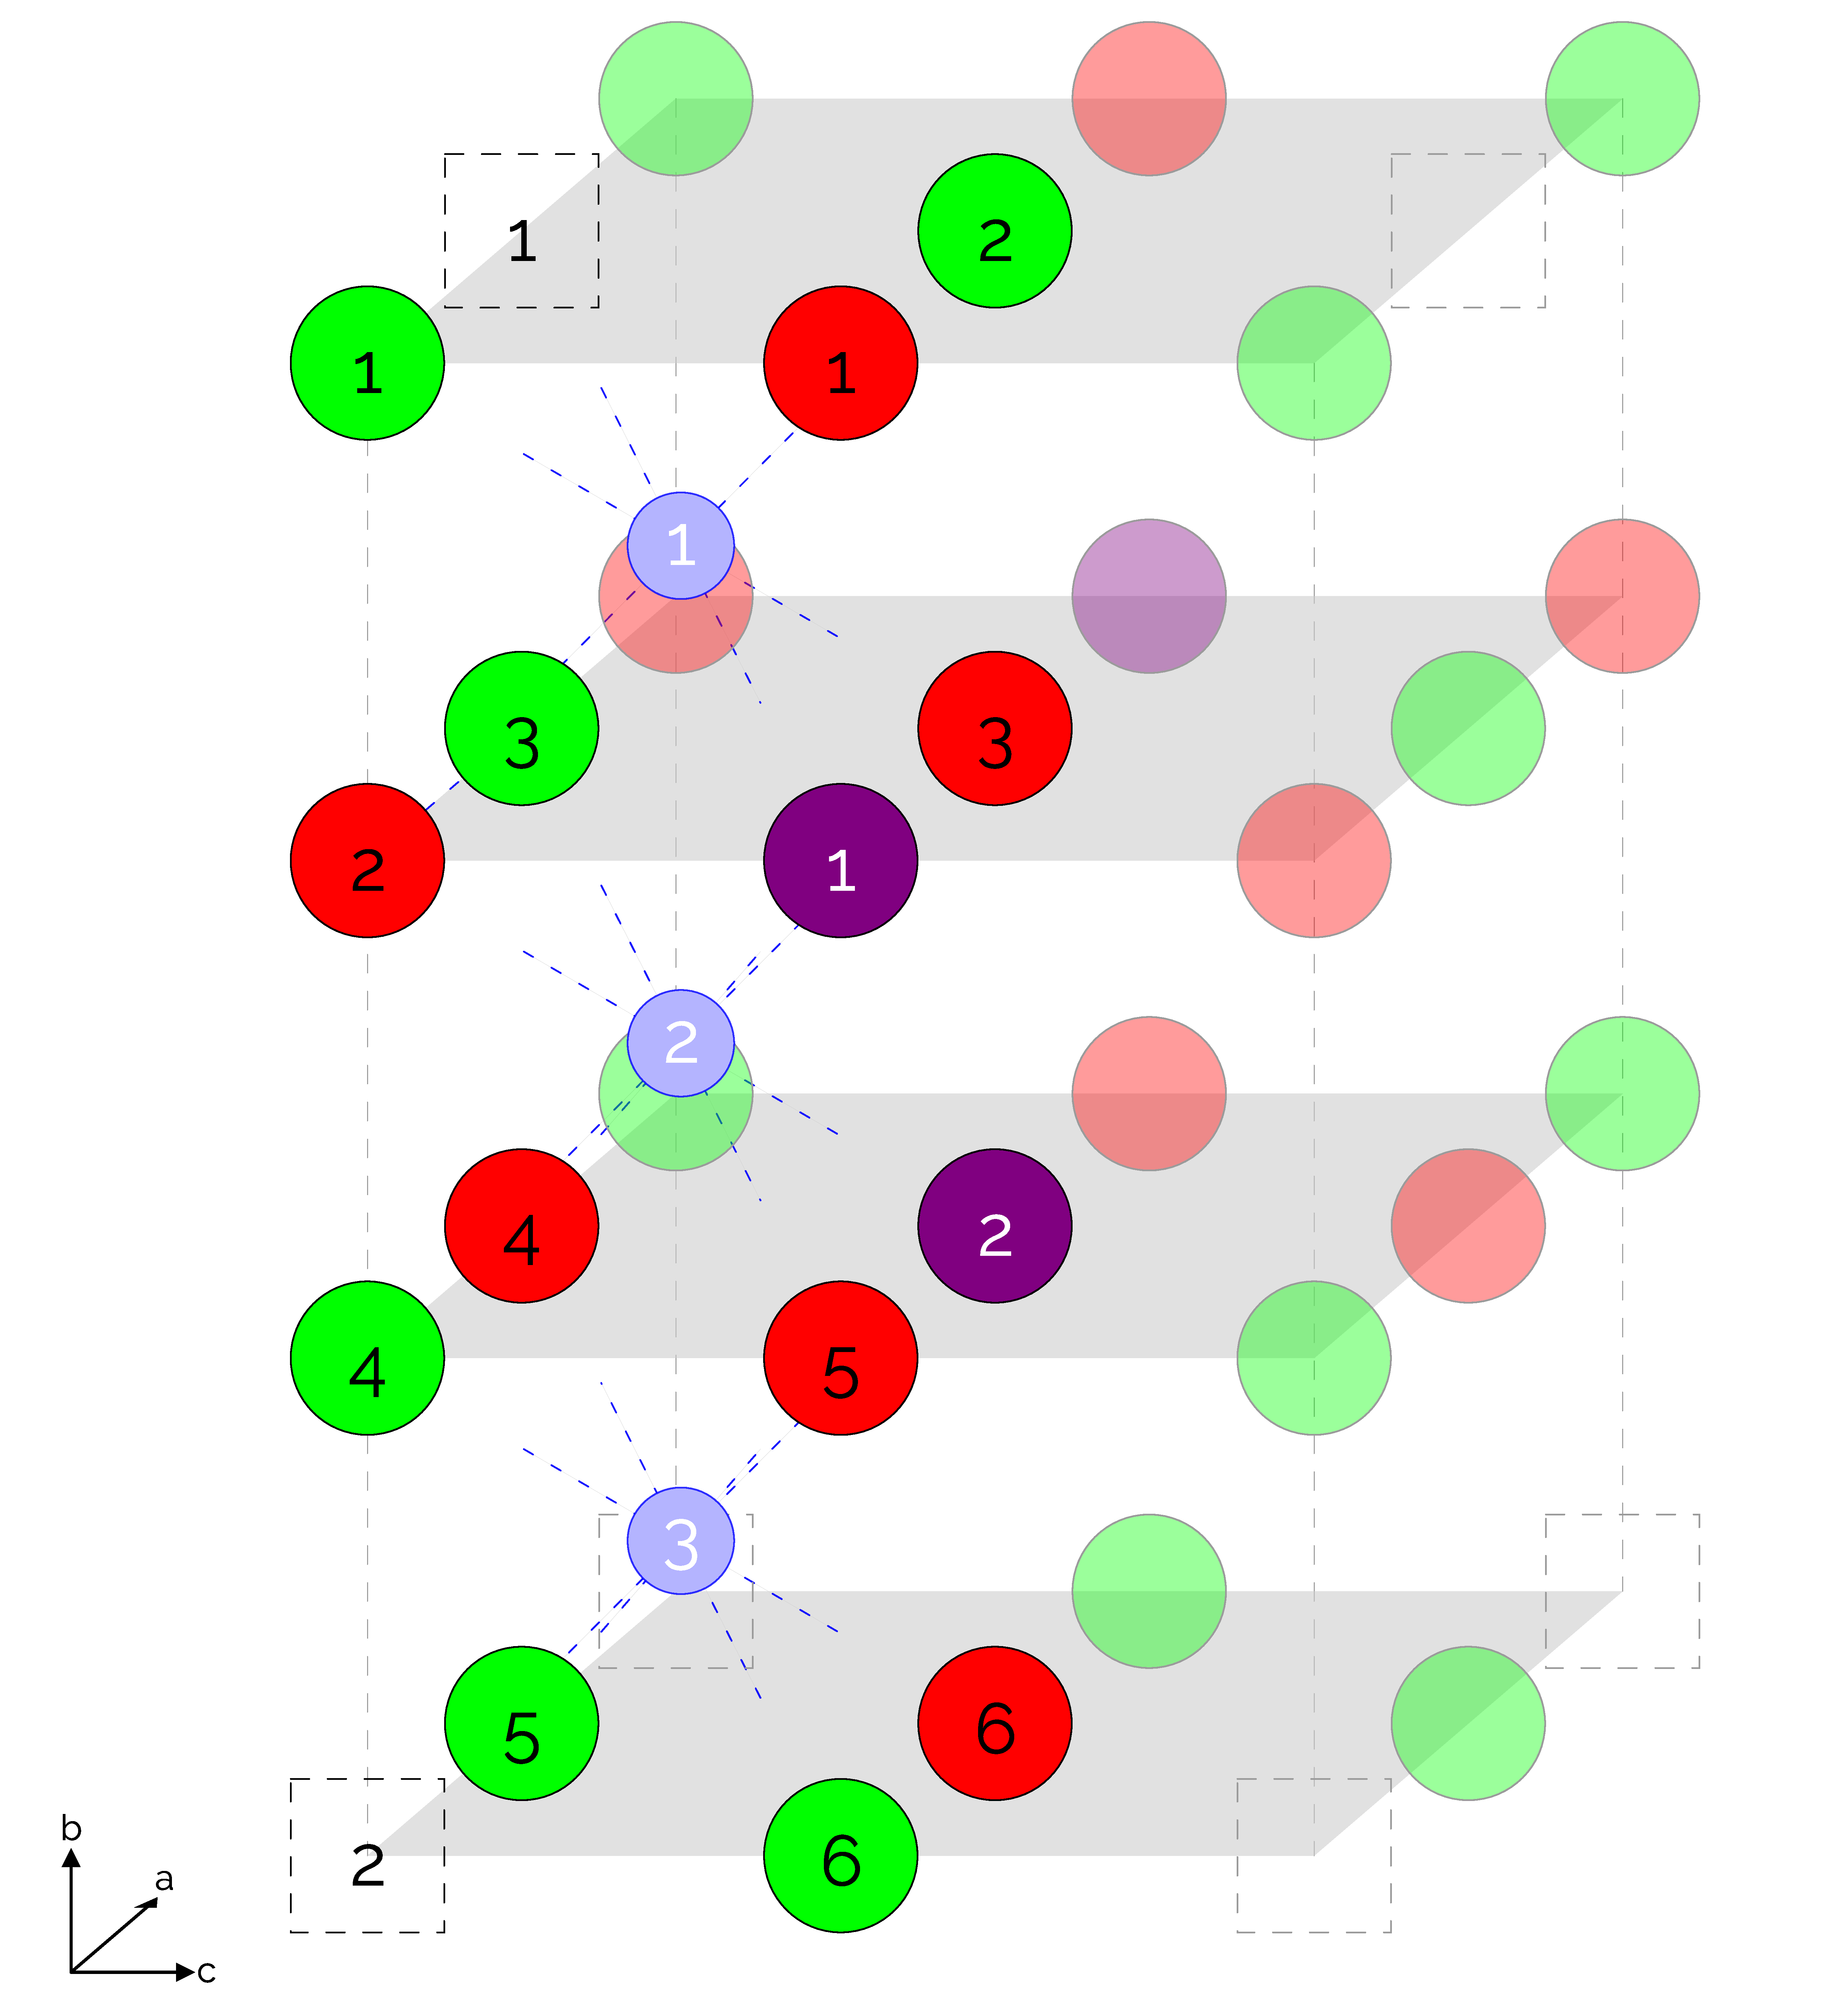
\includegraphics[height = 0.55\textheight]{figures/orderedlabels/orderedlabels}
\caption[Site labelling scheme for ordered \ce{Li4Mn2O5}]{Site labelling scheme for ordered \ce{Li4Mn2O5}. A reflection at either the top or bottom plane yields the structure proposed by \citet{Diaz-Lopez2017}. \\Li ions: green; Mn ions: purple; O atoms: red; O vacancies: dashed squares; Interstitial sites: blue.
}
\label{fig:orderedlabel}
\end{figure}

\section{Intrinsic defects}
Using the ordered structure proposed by \citet{Diaz-Lopez2017}, a series of point defect calculations were calculated, allowing for the formation energies of Schottky, Frenkel, and anti-site defects to be determined.
Figure \ref{fig:orderedlabel} shows the labelling scheme used to refer to each symmetrically unique site in the structure throughout this section.
\newpage
\paragraph{Kr\"oger-Vink notation for \ce{Li4Mn2O5} vacancies}

\begin{align}
\varnothing &\rightarrow \ce{V^\prime_{Li_n}}\\
\varnothing &\rightarrow \ce{V^{\prime \prime \prime}_{Mn_n}}\\
\varnothing &\rightarrow \ce{V^{\bullet\bullet}_{O_n}}
\end{align}
\vfill
\begin{table}[h]
\centering
\caption{Isolated defect energies for the formation of vacancies in \ce{Li4Mn2O5}}
\begin{tabular}{l *{3}{d{2.3}}}
\toprule
&\multicolumn{3}{c}{Species}\\
\cmidrule(lr){2-4}
\textbf{Site (n)} & \mc{\ce{Li}} & \mc{\ce{Mn}} & \mc{\ce{O}}\\
\midrule
1 & 6.931 & 46.193 & 24.771 \\
2 & 5.573 & 46.193 & 23.240 \\
3 & 7.255 & \tableline & 24.612 \\
4 & 7.255 & \tableline & 23.240 \\
5 & 6.931 & \tableline & 24.612 \\
6 & 5.573 & \tableline & 24.771 \\
\midrule
Minimum & 5.573 & 46.193 & 23.240  \\
\bottomrule
\end{tabular}
\label{tab:vacancies}
\end{table}
\vspace{0.25\textheight}
\newpage
\paragraph{Kr\"oger-Vink notation for \ce{Li4Mn2O5} interstitial defects}
\begin{align}
\varnothing &\rightarrow \ce{Li^{\bullet}_{i_n}}\\
\varnothing &\rightarrow \ce{Mn^{\bullet\bullet\bullet}_{i_n}}\\
\varnothing &\rightarrow \ce{O^{\prime \prime}_{i_n}}
\end{align}


\vfill
\begin{table}[h]
\centering
\caption{Isolated defect energies for interstitial defects in \ce{Li4Mn2O5}. Numbered sites 1, 2 and 3 refer to the octohedral sites found between layers 1 and 2, 2 and 3, and 3 and 4 respectively. Sites V1 and V2 refer to vacant O sites.}
\begin{tabular}{l *{3}{d{3.3}}}
\toprule
&\multicolumn{3}{c}{Species}\\
\cmidrule(lr){2-4}
\textbf{Site (n)} & \mc{\ce{Li}} & \mc{\ce{Mn}} & \mc{\ce{O}}\\
\midrule
1 & -3.850 & -36.410 & \tableline \\
2 & -3.799 & -36.712 & -17.087 \\
3 & -3.850 & -36.410 & \tableline \\
V1 & -2.942 & -36.122 & -20.161 \\
V2 & -2.942 & -36.122 & -20.161 \\
\midrule
Minimum & -3.850 & -36.712 & -20.161  \\
\bottomrule
\end{tabular}
\label{tab:interstitial}
\end{table}
\vspace{0.25\textheight}
\newpage

\subsection{Isolated defects}
Tables \ref{tab:vacancies} and \ref{tab:interstitial} show the formation energies of vacancies and interstitial defects at each site labelled in Figure \ref{fig:orderedlabel}.
Oxygen interstitial defects introduced at interstices 1 and 3 migrated into the adjacent oxygen vacancy, with only interstitial site 2 able to host stable interstitial oxygen vacancies.
It is more energetically favourable to introduce oxygen interstitial defects onto the vacant lattice sites.

The formation energy of lithium vacancies differs significantly between sites.
This would lead to these sites being preferentially delithiated.

\subsection{Compound defects}
\begin{table}[h]
\centering
\caption{Schottky defect energies in \ce{Li4Mn2O5}}
\resizebox{\columnwidth}{!}{
\begin{tabular}{l l d{2.3} }
\toprule
\textbf{Type} & \textbf{Formula} & \mc{Formation energy (\si{\electronvolt})}\\
\midrule
Full & $\varnothing \rightarrow \ce{4 V^\prime_{Li} +  3 V^{\prime \prime \prime}_{Mn} + 4V^{\bullet \bullet}_{O} + Li4Mn2O5}$ & 15.11 \\
Li Schottky-like & $\varnothing \rightarrow \ce{2V^\prime_{Li} + V^{\bullet \bullet}_{O} + Li2O} $ & 5.38 \\
Mn Schottky-like & $\varnothing \rightarrow \ce{2V^{\prime \prime \prime}_{Mn} + 3 V^{\bullet \bullet}_{O} + Mn2O3}$ & 5.12 \\
\bottomrule
\end{tabular}
}
\label{tab:schottky}
\end{table}

\begin{table}[h]
\centering
\caption{Frenkel defect energies in \ce{Li4Mn2O5}}
\begin{tabular}{l l d{2.3}}
\toprule
\textbf{Species} & \textbf{Formula} & \mc{Formation energy (\si{\electronvolt})}\\
\midrule
Li & $\varnothing \rightarrow \ce{V^\prime_{Li} +  Li^{\bullet}_{i}}$                               & 1.72 \\
Mn & $\varnothing \rightarrow \ce{V^{\prime \prime \prime}_{Mn} +  Mn^{\bullet\bullet\bullet}_{i}}$ & 9.48 \\
O  & $\varnothing \rightarrow \ce{V^{\bullet\bullet}_{O} +  O^{\prime \prime}_{i}}$                 & 3.08 \\
\bottomrule
\end{tabular}
\label{tab:frenkel}
\end{table}

Tables \ref{tab:schottky} and \ref{tab:frenkel} show the formation energies, for Schottky and Frenkel defects respectively, in \ce{Li4Mn2O5}.
Firstly, the high energies associated with all the defects tabulated shows that the concentration of all such defects will be very low in the fully lithiated system.
The most favourable, a Li Frenkel defect, would likely be unstable in a partially delithiated structure where few interstitial sites not adjacent to a Li vacancy would exist.
The relatively low energy of the second most favourable defect type, O Frenkel, can be attributed to the presence of vacant O sites throughout the rock-salt structure.

\newpage


\section{Migration energetics and pathways}
\label{sec:migration}
\begin{table}[h]
\centering
\caption{Li vacancy migration energies in \ce{Li4Mn2O5} in eV.}

\begin{tabular}{c *{6}{d{3.4}}}
\toprule
& \multicolumn{6}{c}{Final site} \\
\cmidrule(lr){2-7}
Initial site & \mc{1}     & \mc{2}     & \mc{3}     & \mc{4}     & \mc{5}     & \mc{6}     \\ \midrule
1            & \tableline & 0.32       & 1.68       & \tableline & \tableline & \tableline \\   
2            & 1.68       & \tableline & 2.13       & \tableline & \tableline & \tableline \\
3            & 1.29       & 0.45       & \tableline & 0.61       & \tableline & \tableline \\
4            & \tableline & \tableline & 0.61       & \tableline & 1.29       & 0.45       \\
5            & \tableline & \tableline & \tableline & 1.61       & \tableline & 1.61       \\
6            & \tableline & \tableline & \tableline & 2.13       & 1.68       & \tableline \\
\bottomrule
\end{tabular}

\label{tab:migrationMn}
\end{table}




\newpage
\section{Dynamics study}
\newpage